\section{数据预处理实现及结果分析}
在本文,将依次按照数据准备、数据清洗、数据变换、数据聚合以及特征值构造和维度规约的顺序对所挖掘数据集进行转换。

\subsection{数据准备}
首先针对每一张表进行冗余数据的校验处理,删掉重复项。比如在有些表中会有相同的元组数据,这就可以删除。

此过程借助于Navicat工具的自动排序功能,简化了原始数据集,有利于进一步对数据进行处理。

此外,依据inf这张表,设置age过滤范围,并以此确认age位于18到70之间。

通过上述数据限定范围,对inf表进行范围限定处理。

\subsection{数据清洗—数据集缺失值的处理}
在本文中,本文中主要采用两类处理方法来对表中出现的缺失值进行处理。首先通过对数据录入时的限制函数对指定的录入数据类进行限制,然后在数据读取后对非必需类数据进行统一缺省处理。

\subsubsection{user数据集中缺失值的处理:}
观察inf有关数据集,我们发现user相关数据属性出现缺失值现象:

主要集中在读入数据的No.10~No.25:

\begin{figure}[thbp!]
	\centering
	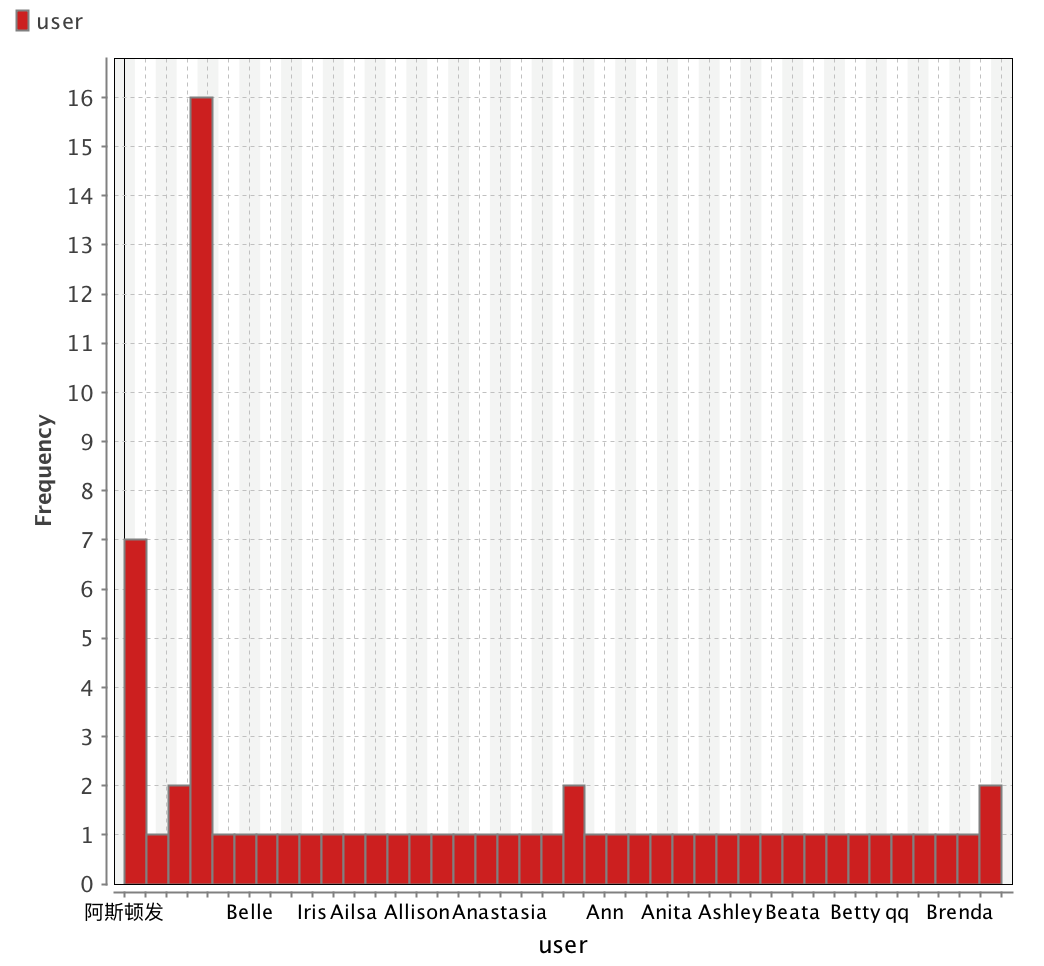
\includegraphics[width=0.4\linewidth]{figure/5-1}
	\caption{缺失值现象}
	\label{fig:5-1}
\end{figure}

观察数据,可以发现图5-1中Belle这个user前的16个样本为空样本。

现在,做一下几个工作:

\begin{itemize}
	\item 首先,添加Filter Examples 算子到Process;
	\item 其次,添加Entry;
\end{itemize}

设置user属性 is not in,即过滤掉读入的user属性为缺省的数据项。

现在,给出此次过滤后的图5-2:

\begin{figure}[thbp!]
	\centering
	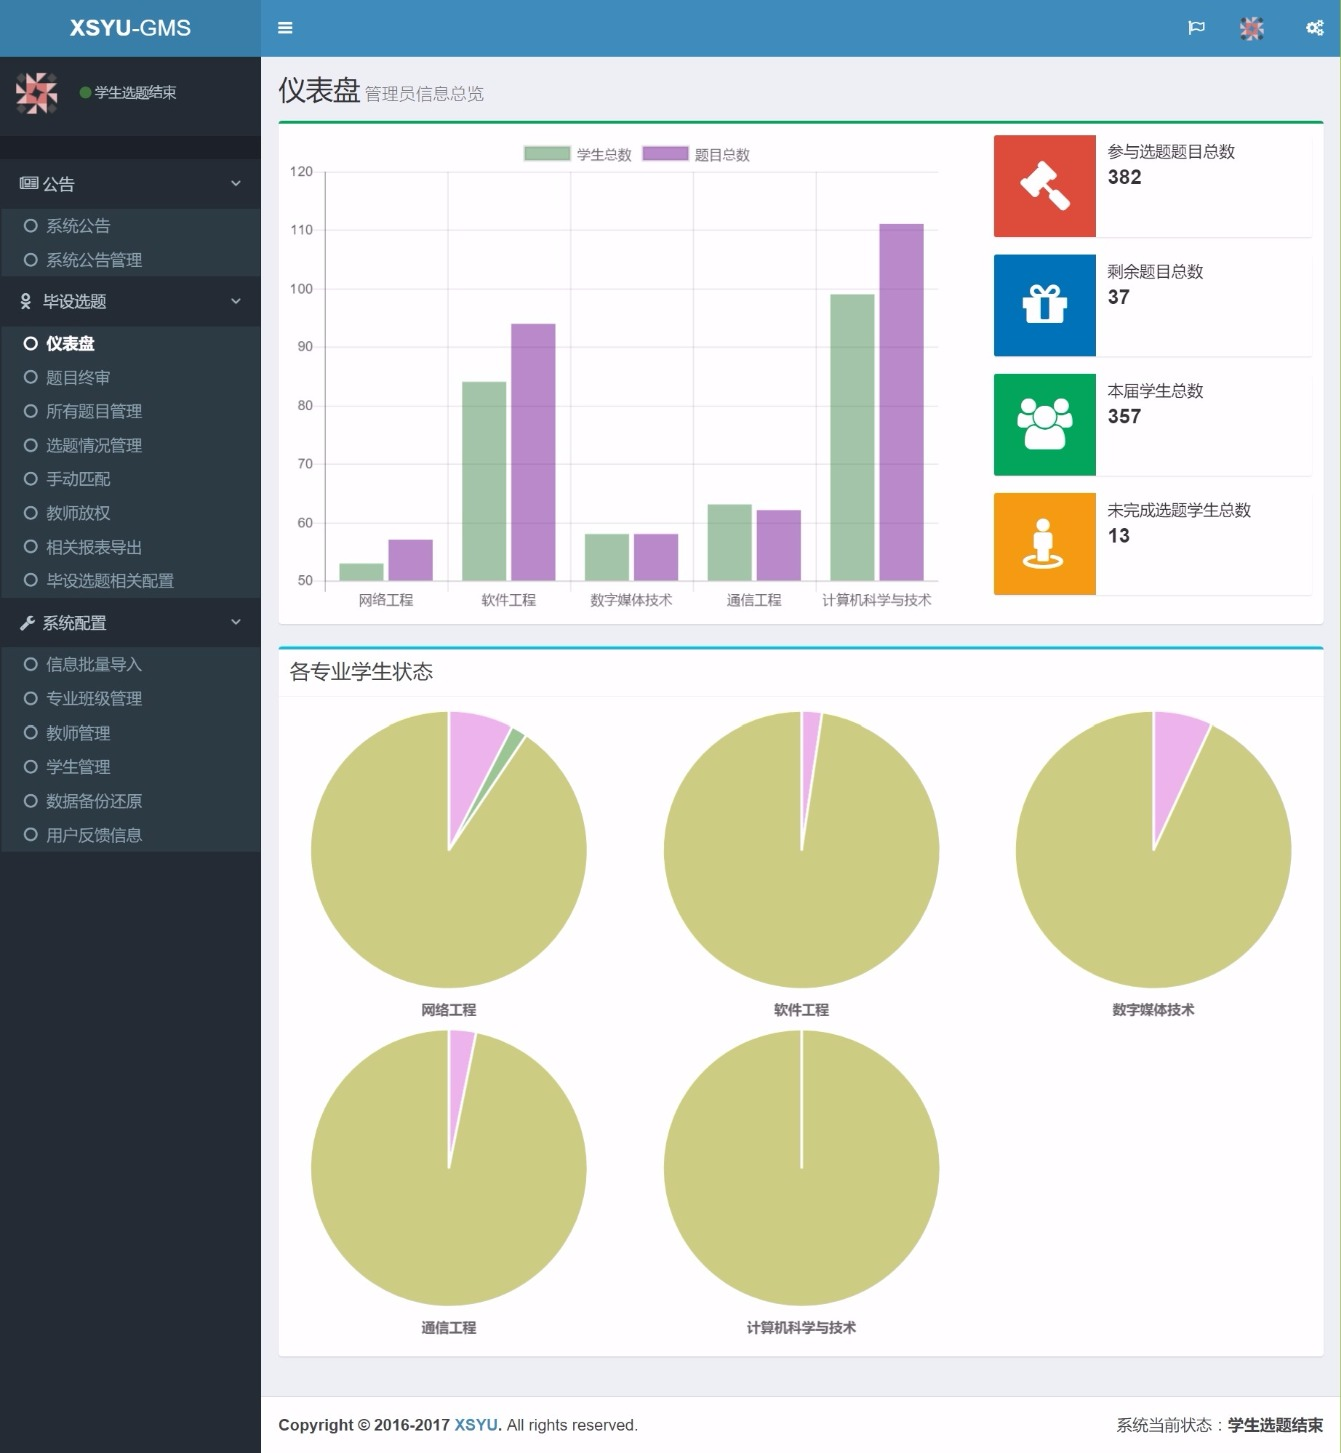
\includegraphics[width=0.4\linewidth]{figure/5-2}
	\caption{过滤后的图片}
	\label{fig:5-2}
\end{figure}

观察上述分布图5-2,会发现user缺失值的已经全部处理完成。

\subsubsection{ 年龄的处理}
观察用户信息有关数据集,会发现与用户年龄数据属性出现异常现象,主要在在inf表,其中有以下几个字段出现丢失值现象:

 首先,分析以下分布图5-3:
 
 \begin{figure}[thbp!]
 	\centering
 	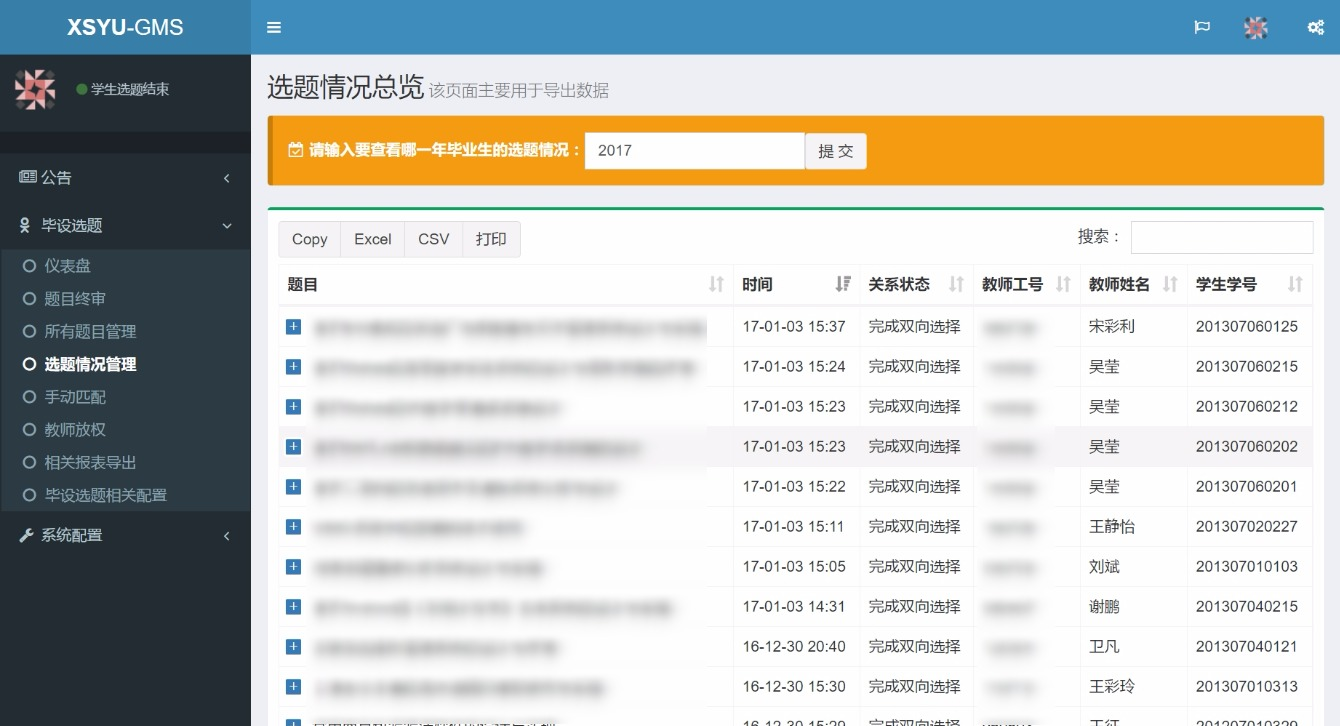
\includegraphics[width=0.4\linewidth]{figure/5-3}
 	\caption{age分布图}
 	\label{fig:5-3}
 \end{figure}

简要的对此属性值出现的情况做一简单统计:

<18的,即FALSE,有6人;

>=18且<=70,即TRUE,有42人;

设置Filter Examples算子,添加age过滤条件过滤不符合的数据,如图5-4:

\begin{figure}[thbp!]
	\centering
	\includegraphics[width=0.4\linewidth]{figure/5-4}
	\caption{添加age过滤条件}
	\label{fig:5-4}
\end{figure}

保存后运行算法,因此,得出age过滤后的图像,如图5-5:

\begin{figure}[thbp!]
	\centering
	\includegraphics[width=0.4\linewidth]{figure/5-5}
	\caption{过滤后的图}
	\label{fig:5-5}
\end{figure}

如图,age不符合条件的数据已经全部处理完成

\subsubsection{ 关于专业的预处理}

经过前面对数据集的相关的处理,观察到有关专业的数据还存在有异常项,如图5-6所示:

\begin{figure}[thbp!]
	\centering
	\includegraphics[width=0.4\linewidth]{figure/5-6}
	\caption{专业预处理前}
	\label{fig:5-6}
\end{figure}

\newpage
很显然可以从图5-6看出存在两个属性值的发售地方与苏打粉撒的为异常属性值,因此我们同样采取Filter Examples算子,设置过滤条件如图5-7:

\begin{figure}[thbp!]
	\centering
	\includegraphics[width=0.4\linewidth]{figure/5-7}
	\caption{设置过滤条件}
	\label{fig:5-7}
\end{figure}

保存后运行算子得到输出的major数据分布如图5-8:

\begin{figure}[thbp!]
	\centering
	\includegraphics[width=0.4\linewidth]{figure/5-8}
	\caption{工种预处理后的数据集合}
	\label{fig:5-8}
\end{figure}

由此,我们就得到了所有数据预处理后的数据集合,总计40 examples。


\subsection{数据变换}
根据任务书要求,从工种和驻地以及文化程度这三个方面来对数据集进行数据变换处理。

\subsubsection{关于驻地的相关数据处理及决策树生成}

经过前面对数据集的相关的处理,得到了40条合理的数据集,接下来,依次对每个属性进行具体的相关分析。

(1)设置关联属性;

观察表中数据,选取工种、驻地、文化程度三个属性设置相关,实现聚类。

具体做法:

首先,利用RapidMiner工具,使用Read Database读入数据库数据;

其次,利用Filter Examples完成数据预处理;

然后,利用Select Attributes选择所需三个属性,如图5-9:

\begin{figure}[thbp!]
	\centering
	\includegraphics[width=0.4\linewidth]{figure/5-9}
	\caption{选择所需三个属性}
	\label{fig:5-9}
\end{figure}

设置好算子后运行可见,数据charts如图5-10:

\begin{figure}[thbp!]
	\centering
	\includegraphics[width=0.4\linewidth]{figure/5-10}
	\caption{数据charts}
	\label{fig:5-10}
\end{figure}

x轴代表工种属性,y轴代表文化程度属性,z轴代表驻地属性,通过Sticks 3D图像来表示出数据分布

(2)对所选数据设置处理规则

选用Set Role算子,对 major, status, residence 三个属性分别设置处理规则如图5-11:

\begin{figure}[thbp!]
	\centering
	\includegraphics[width=0.4\linewidth]{figure/5-11}
	\caption{设置处理规则}
	\label{fig:5-11}
\end{figure}

目的为将文化程度设置为label,工种跟驻地设置为regular

处理结果如图5-12:

\begin{figure}[thbp!]
	\centering
	\includegraphics[width=0.4\linewidth]{figure/5-12}
	\caption{处理结果}
	\label{fig:5-12}
\end{figure}

如图5-12可见我们已经将文化程度设置为label,工种跟驻地设置为regular

(3)生成驻地决策树

运用Decision Tree算子,通过对label status属性,regular major, residence属性进行决策树生成如图5-13:

\begin{figure}[thbp!]
	\centering
	\includegraphics[width=0.4\linewidth]{figure/5-13}
	\caption{驻地决策树}
	\label{fig:5-13}
\end{figure}

从图5-13可以看出经过数据分析后,不同的驻地导向了不同的文化程度,比如:驻地为乡镇就导向小学文化程度。

 Tree 

residence = County, county-level city, city area: high-school-educated

 \{Bachelor degree or above=0, primary-school-educated=0, Undergraduate-educated=0, high-school-educated=9\}
residence = State / Province: Bachelor degree or above 

\{Bachelor degree or above=10, primary-school-educated=2, Undergraduate-educated=9, high-school-educated=0\}
residence = Township, town: primary-school-educated 

\{Bachelor degree or above=0, primary-school-educated=10, Undergraduate-educated=0, high-school-educated=0\}

\subsubsection{关于工种的相关数据处理及决策树生成}
经过前面对数据集的相关的处理,得到了40条合理的数据集,接下来,依次对每个属性进行具体的相关分析。

(1)设置关联属性;

观察表中数据,选取工种、驻地、文化程度三个属性设置相关,实现聚类

具体做法:

首先,利用RapidMiner工具,使用Read Database读入数据库数据;

其次,利用Filter Examples完成数据预处理;

 然后,利用Select Attributes选择所需三个属性,如图5-14:
 
 \begin{figure}[thbp!]
 	\centering
 	\includegraphics[width=0.4\linewidth]{figure/5-14}
 	\caption{设置关联属性}
 	\label{fig:5-14}
 \end{figure}

选择工种,驻地,文化程度为所需的三个属性

设置好算子后运行可见,数据charts如图5-14:

\begin{figure}[thbp!]
	\centering
	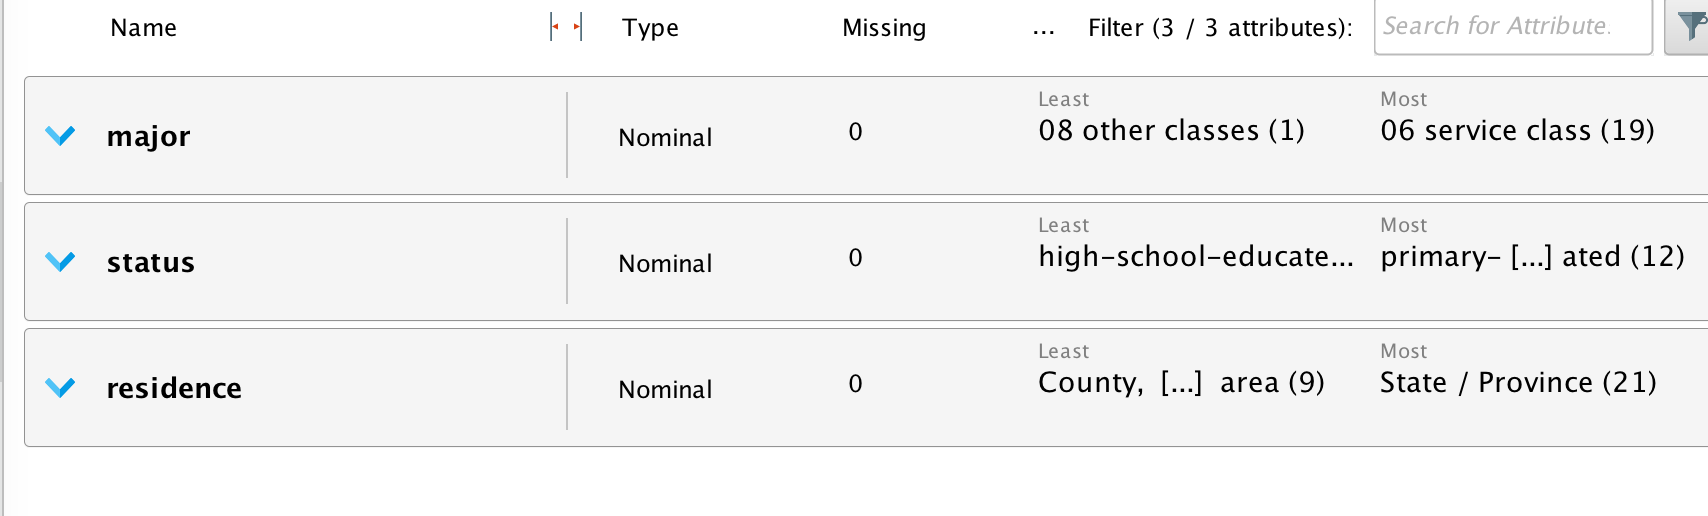
\includegraphics[width=0.4\linewidth]{figure/5-15}
	\caption{数据charts}
	\label{fig:5-15}
\end{figure}

如图5-15,我们所选择的工种,驻地,文化程度三个属性已经被挑选出来。

(2)对所选数据设置处理规则

选用Set Role算子,对 major, status, residence 三个属性分别设置处理规则如图5-16:

\begin{figure}[thbp!]
	\centering
	\includegraphics[width=0.4\linewidth]{figure/5-16}
	\caption{设置处理规则}
	\label{fig:5-16}
\end{figure}

目的为将工种设置为label,文化程度跟驻地设置为regular。

处理结果如图5-17:

\begin{figure}[thbp!]
	\centering
	\includegraphics[width=0.4\linewidth]{figure/5-17}
	\caption{处理结果}
	\label{fig:5-17}
\end{figure}

如图5-17可见,我们已经将工种设置为label,文化程度跟驻地设置为regular。

(3)生成工种决策树

运用Decision Tree算子,通过对label major属性,regular status, residence属性进行决策树生成如图5-18:

\begin{figure}[thbp!]
	\centering
	\includegraphics[width=0.4\linewidth]{figure/5-18}
	\caption{工种决策树}
	\label{fig:5-18}
\end{figure}

如图5-18可见,不同的工种经过数据处理后对应到不同的学历及驻地,衍生出对应规则。如:02 管理工种就对应本科文化程度,省级驻地

Tree 

residence = County, county-level city, city area: 06 service class {08 other classes=0, 07 high-tech category=0, 06 service class=9, 02 management=0}
residence = State / Province

|   status = Bachelor degree or above: 07 high-tech category {08 other classes=1, 07 high-tech category=9, 06 service class=0, 02 management=0}

|   status = Undergraduate-educated: 02 management {08 other classes=0, 07 high-tech category=0, 06 service class=0, 02 management=9}

|   status = primary-school-educated: 07 high-tech category {08 other classes=0, 07 high-tech category=1, 06 service class=0, 02 management=1}

residence = Township, town: 06 service class {08 other classes=0, 07 high-tech category=0, 06 service class=26, 02 management=0}
